\documentclass[11pt,a4paper]{article}
\usepackage[margin=2.5cm]{geometry}
\usepackage{booktabs}
\usepackage{listings}
\usepackage{xcolor}
\usepackage{graphicx}
\usepackage{float}

\lstset{
  basicstyle=\ttfamily\small,
  frame=single,
  backgroundcolor=\color{gray!8},
  breaklines=true
}

\title{Labwork 7: Reduction}
\author{Yanis Denizot -- 2640051}
\date{\today}

\begin{document}
\maketitle

\section{Implementation}
The grayscale stretch has 3 steps: convert to gray (map), find the min and max intensity
(reduce), then recompute each pixel from $[min, max]$ to $[0, 255]$ (map):
\[
g' = \frac{(g - min) \times 255}{max - min}
\]
A normal photo already has values from 0 to 255, so the stretch would do nothing. To see the
effect, I first made a low contrast version of the image with \texttt{img * 0.4 + 80}, so the
values are between 80 and 182. The image is $1200 \times 800$ and I used Google Colab (Tesla T4).

The gray and stretch kernels are 2D map kernels like in labwork 6. I used integer division
(\texttt{//}) to avoid float64, which is slow on the T4 (see labwork 6).

\textbf{Reduction.} The min/max kernel works on the flattened gray image. Each block copies its
values into shared memory, then does the reduction like in the course (``Optimize: Final''
version): at each step, the first half of the threads compare their value with the value
\texttt{s} positions further, and \texttt{s} is divided by 2. I compute the min and the max at
the same time, in two shared arrays. The threads outside the image put neutral values (255 for
the min and 0 for the max), so they never change the result.

\begin{lstlisting}[language=Python]
s = cuda.blockDim.x // 2
while s > 0:
    if tid < s:
        sMin[tid] = min(sMin[tid], sMin[tid + s])
        sMax[tid] = max(sMax[tid], sMax[tid + s])
    cuda.syncthreads()
    s = s // 2
if tid == 0:
    dstMin[cuda.blockIdx.x] = sMin[0]
    dstMax[cuda.blockIdx.x] = sMax[0]
\end{lstlisting}

Each block gives one min and one max, so I launch the kernel again on the results of the
previous pass, until only one value is left. For example with 256 threads per block:
$960\,000 \rightarrow 3750 \rightarrow 15 \rightarrow 1$. The final min and max are copied
to the CPU and given to the stretch kernel. The block size must be a power of 2 for the
reduction.

The GPU finds the same min and max as the CPU (80 and 182), and the stretched image is the
same as the CPU result (maximum difference = 0).

\begin{figure}[H]
\centering
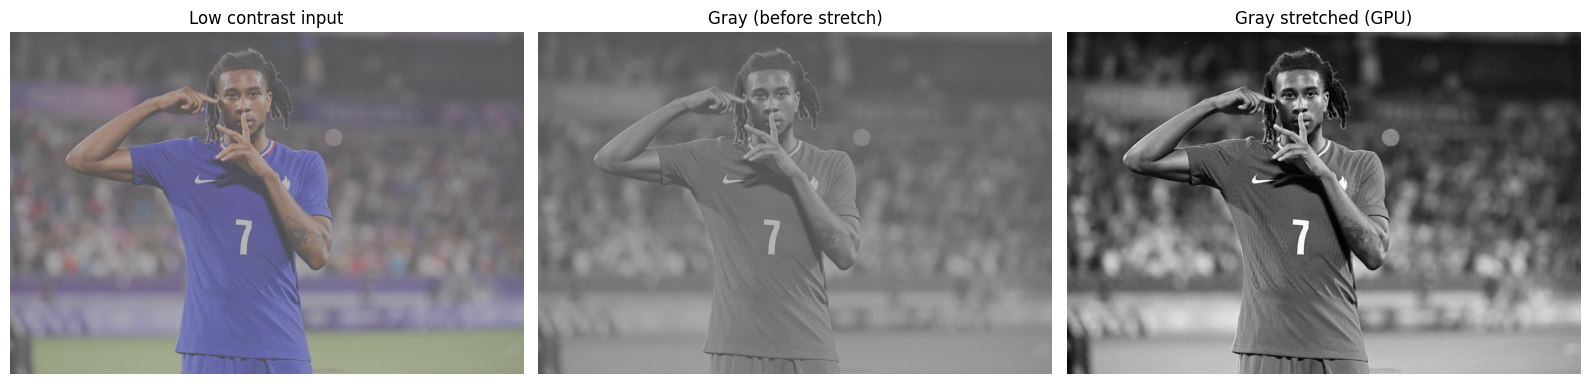
\includegraphics[width=\textwidth]{results.png}
\end{figure}

\section{Block size}
The CPU version (Python loops for the 3 steps) takes 2.02 s. The GPU time is the average of
20 runs of the full pipeline (gray + min/max + stretch). For the reduction I use 1D blocks with
the same number of threads as the 2D blocks.

\begin{table}[H]
\centering
\begin{tabular}{lrrr}
\toprule
Block & Reduction passes & GPU time (ms) & Speedup \\
\midrule
$8 \times 8$ (64)     & 4 & 2.03 & 996 \\
$16 \times 8$ (128)   & 3 & 1.33 & 1518 \\
$16 \times 16$ (256)  & 3 & 0.96 & 2106 \\
$32 \times 16$ (512)  & 3 & 0.94 & 2139 \\
$32 \times 32$ (1024) & 2 & 0.74 & 2722 \\
\bottomrule
\end{tabular}
\end{table}

\begin{figure}[H]
\centering
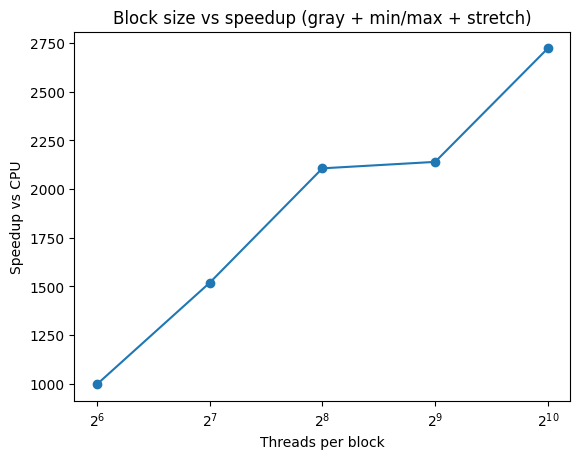
\includegraphics[width=0.65\textwidth]{blocksize_vs_speedup.png}
\end{figure}

Here, unlike the previous labworks, the biggest blocks are the fastest. I think this is because
the gray and stretch kernels are very fast (tens of $\mu$s in labwork 6), so the time is mostly
the overhead of the reduction: each pass needs a new kernel launch and two new arrays on the
GPU. With bigger blocks there are fewer passes (2 with 1024 threads, 4 with 64 threads), and the
first pass also writes fewer results. Numba also gives a warning for the last passes, because
they have only a few blocks (for example 1 or 4), which uses only a small part of the GPU.
A possible optimization would be to allocate the arrays only once, outside the measured loop.

\end{document}
